\section{Tulokset}

Kuvassa \ref{fig:music} on simuloitu MUSIC-algoritmia sekä kiinteällä että vapaalla orientaatiolla. Simuloinneissa kolme lähdedipolia sijoitettiin aivokuorelle, jotka on merkitty punaisina ympyröinä ja topografia on muodostettu MUSIC-algoritmin paikannusfunktion arvoista.

Kuvissa \ref{fig:RAPfix} ja \ref{fig:RAPfree} on simuloitu RAP-MUSIC- algoritmia kiinteällä ja vapaalla orientaatiolla. Kuvissa musta rasti kuvaa paikannusfunktion maksimiarvon paikkaa ja löydetyt dipolit merkataan punaisella neliöllä. Vastaavasti kuvissa \ref{fig:TRAPfix} ja \ref{fig:TRAPfree} on kuvattu TRAP-MUSIC:n käyttöä kiinteällä ja vapaalla orientaatiolla. 

Kuvista huomataan, että MUSIC vapaalla orientaatiolla saa aikaan suurempia aktiivisuuden alueita kuin kiinteällä orientaatiolla, mikä vaikeuttaa lähteiden tarkkaa paikantamista. 

Tavallisen MUSIC-algoritmin yksi ongelmista on oikeiden lähteiden erottaminen vääristä \citep{Mosher1998RecursiveLocalization}. Oikeiden lähteiden löytäminen kuvasta voi olla vaikeaa, kun lähteiden määrä on suuri. Lisäksi MUSIC-algoritmilla on vaikeuksia löytää synkronoituja lähteitä \citep{Mosher1999SourceMUSIC}. Kaikilla MUSIC-algoritmin versioilla on vaikeuksia löytää hyvin lähellä toisiaan olevia dipoleita. RAP- ja TRAP-MUSIC:ssa löydettyä lähdettä projisoidessa pois häviää myös löytämättä jääneen lähteen topografiaa, jolloin viereistä lähdettä ei välttämättä löydetä.

\begin{figure}[hb]
    \begin{minipage}{0.5\textwidth}
        \centering
        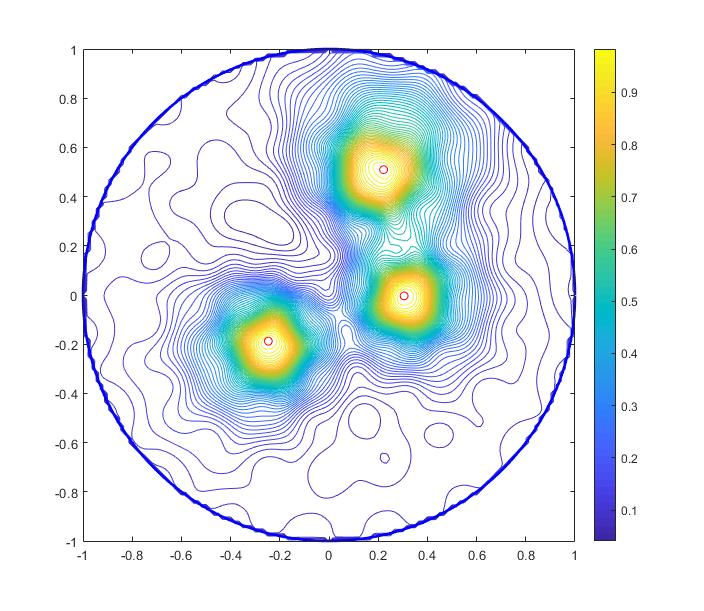
\includegraphics[width=\textwidth]{mfix.jpg} 
    \end{minipage}
    \begin{minipage}{0.5\textwidth}
        \centering
        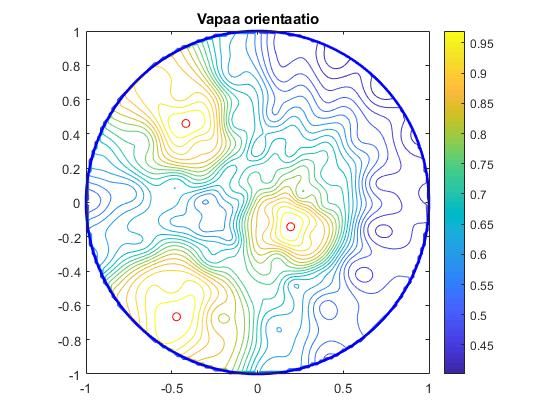
\includegraphics[width=\textwidth]{mfree.jpg}
    \end{minipage}
    \caption{MUSIC-algoritmilla piirretyt topografiakuvat. Vasemmalla puolella orientaatio on kiinteä ja oikealla vapaa.}
    \label{fig:music}
\end{figure}

\clearpage

\begin{figure}[ht]
    \centering
    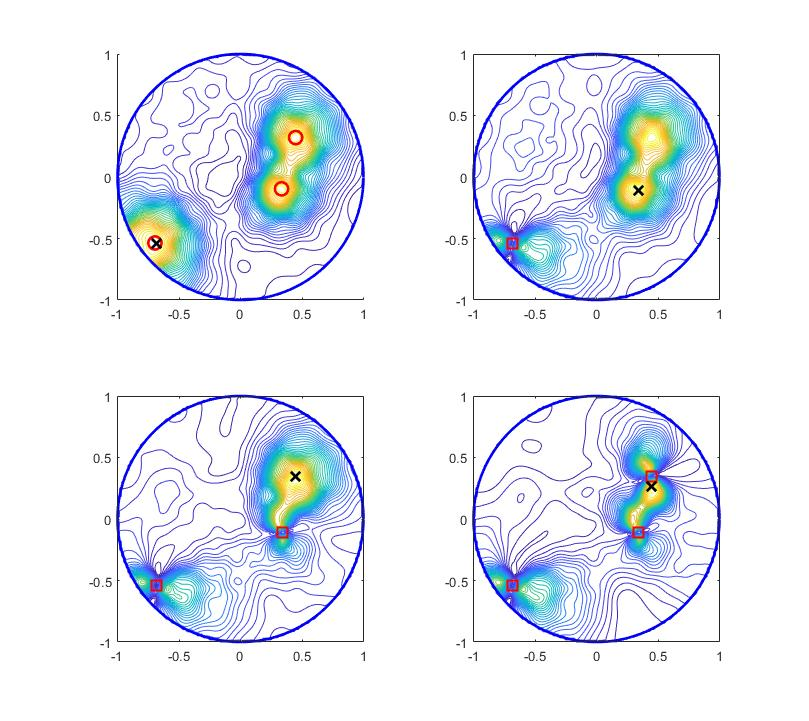
\includegraphics[width=0.7\textwidth]{RAPfixed.jpg}
    \caption{RAP-MUSIC kiinteällä orientaatiolla}
    \label{fig:RAPfix}
\end{figure}

\begin{figure}[h!]
    \centering
    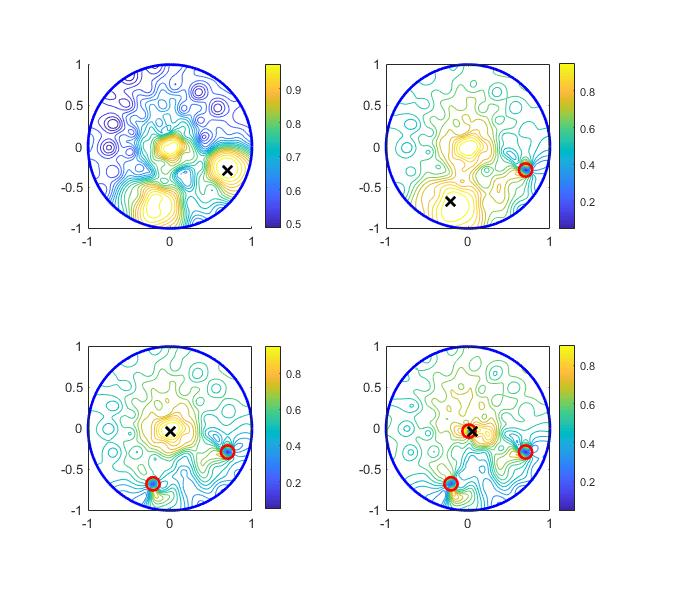
\includegraphics[width=0.7\textwidth]{RAPfree.jpg}
    \caption{RAP-MUSIC vapaalla orientaatiolla}
    \label{fig:RAPfree}
\end{figure}

\clearpage
\begin{figure}[ht]
    \centering
    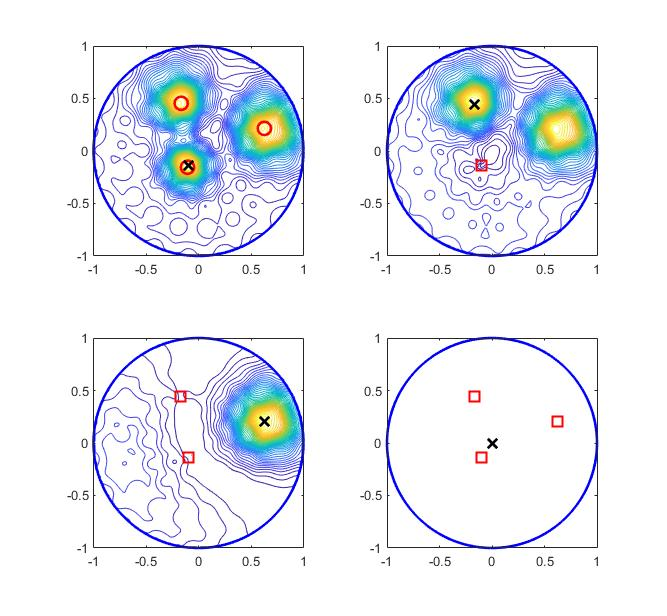
\includegraphics[width = 0.65\textwidth]{trap.jpg}
    \caption{TRAP-MUSIC kiinteällä orientaatiolla}
    \label{fig:TRAPfix}
\end{figure}

\begin{figure}[h!]
    \centering
    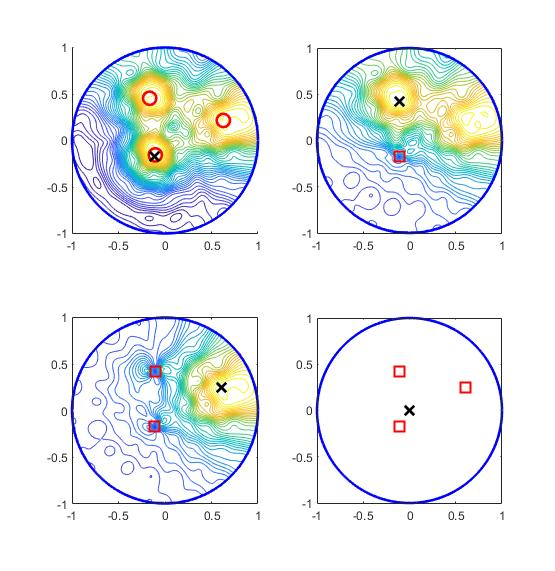
\includegraphics[width = 0.65\textwidth]{trapp.jpg}
    \caption{TRAP-MUSIC vapaalla orientaatiolla}
    \label{fig:TRAPfree}
\end{figure}

\clearpage
\begin{figure}[h]
    \begin{minipage}{0.5\textwidth}
        \centering
        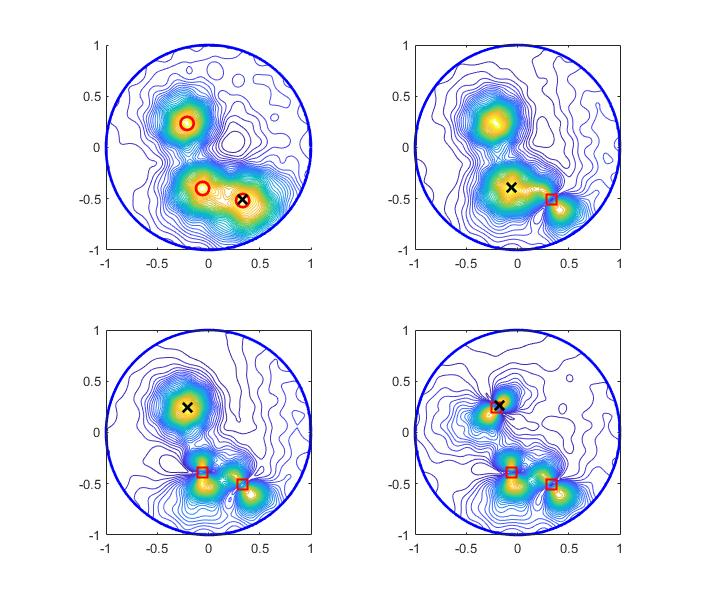
\includegraphics[width=\textwidth]{raptrap2.jpg} 
    \end{minipage}
    \begin{minipage}{0.5\textwidth}
        \centering
        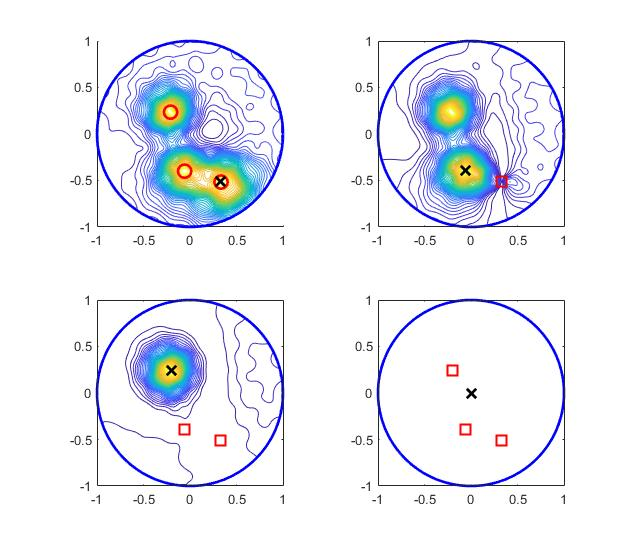
\includegraphics[width=\textwidth]{raptrap1.jpg}
    \end{minipage}
    \caption{RAP- ja TRAP-MUSIC:n vertausta.}
\end{figure}

\clearpage

\begin{figure}
    \centering
    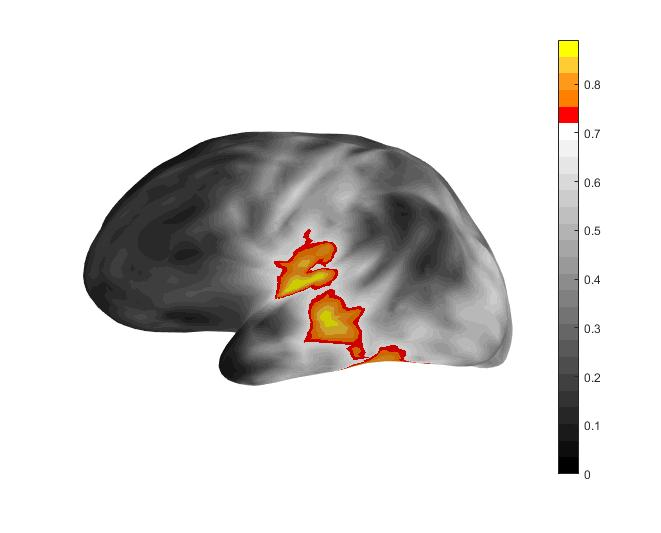
\includegraphics[width=0.7\textwidth]{kuulo.jpg}
    \caption{Kuva oikeiden aivojen mallilla vektori:MUSIC:lla. Kyseessä on kuuloärsykkeestä aiheutunut aktivaatio kuuloaivokuorella.}
\end{figure}

\begin{figure}
    \centering
    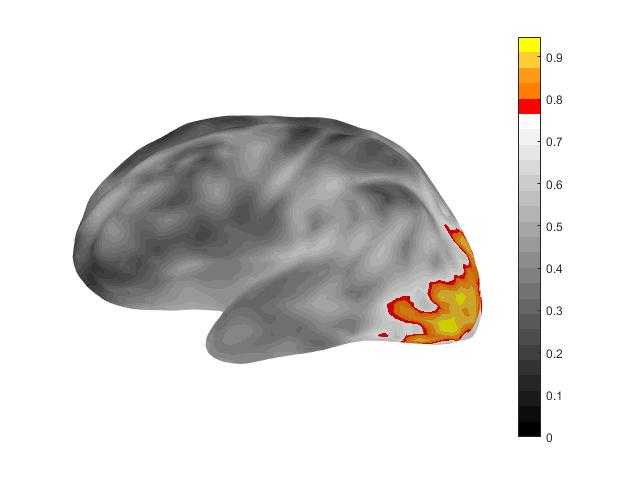
\includegraphics[width=0.7\textwidth]{esim1.jpg}
    \caption{Näköärsykkeestä aiheutunut aktivaatio havaittu näköaivokuorella.}
\end{figure}